\begin{figure}[h]
    \centering
    \begin{subfigure}[b]{0.70\textwidth}
        \centering
        \input{Bilder/Auswertung/VglMessmeth/VglMessmethrefl500adn5000.tex}
        \caption{$Reflectance$}
        \label{fig:y equals x}
    \end{subfigure}  
    

    \begin{subfigure}[b]{0.70\textwidth}
        \centering
        \input{Bilder/Auswertung/VglMessmeth/VglMessmethtrans500adn5000.tex}   
        \caption{$Transmission$} 
        \label{fig:three sin x}
    \end{subfigure}

    \caption{Spectra measured in reflectance and transmission on a thin film of PS on Glass. The films are coated with different coating speeds.}
    \label{fig:SpecRefTrans}
\end{figure}


\begin{figure}[h]
    \centering


    \vspace{1cm}
    \begin{subfigure}[b]{\textwidth}
        \centering
        % This file was created with tikzplotlib v0.10.1.
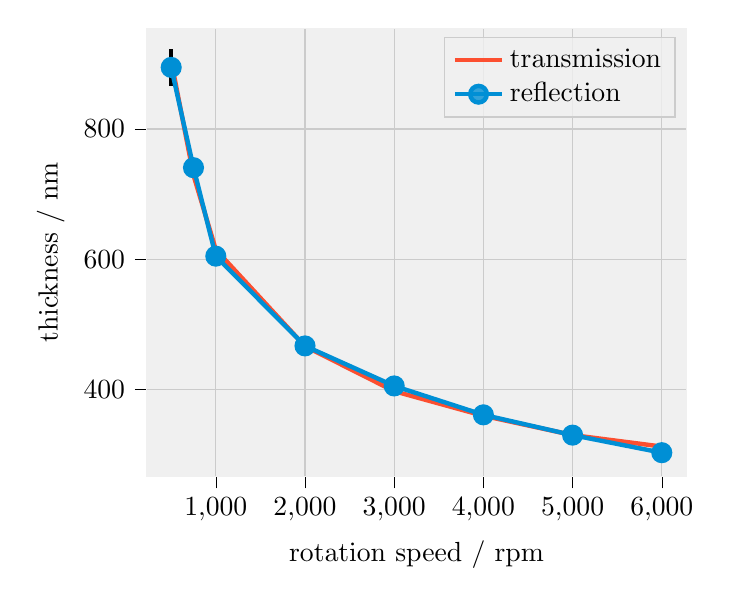
\begin{tikzpicture}

\definecolor{dodgerblue0143213}{RGB}{0,143,213}
\definecolor{lightgray203}{RGB}{203,203,203}
\definecolor{lightgray204}{RGB}{204,204,204}
\definecolor{tomato2527948}{RGB}{252,79,48}
\definecolor{whitesmoke240}{RGB}{240,240,240}

\begin{axis}[
axis background/.style={fill=whitesmoke240},
axis line style={whitesmoke240},
legend cell align={left},
legend style={fill opacity=0.8, draw opacity=1, text opacity=1, draw=lightgray204, fill=whitesmoke240},
tick align=outside,
tick pos=left,
x grid style={lightgray203},
xlabel={rotation speed / rpm},
xmajorgrids,
xmin=225, xmax=6275,
xtick style={color=black},
y grid style={lightgray203},
ylabel={thickness / nm},
ymajorgrids,
ymin=266.056164037744, ymax=954.733300161791,
ytick style={color=black}
]
\path [draw=black, ultra thick]
(axis cs:500,865.670206025666)
--(axis cs:500,923.429793974334);

\path [draw=black, ultra thick]
(axis cs:750,732.309509938563)
--(axis cs:750,748.657156728103);

\path [draw=black, ultra thick]
(axis cs:1000,599.244317659408)
--(axis cs:1000,609.955682340592);

\path [draw=black, ultra thick]
(axis cs:2000,459.903097688354)
--(axis cs:2000,473.530235644979);

\path [draw=black, ultra thick]
(axis cs:3000,398.026298881297)
--(axis cs:3000,412.407034452037);

\path [draw=black, ultra thick]
(axis cs:4000,353.366740906085)
--(axis cs:4000,368.333259093915);

\path [draw=black, ultra thick]
(axis cs:5000,314.740329019556)
--(axis cs:5000,344.593004313777);

\path [draw=black, ultra thick]
(axis cs:6000,297.359670225201)
--(axis cs:6000,308.006996441466);

\addplot [ultra thick, tomato2527948]
table {%
500 904.45
750 729.066666666667
1000 614.6
2000 466.166666666667
3000 397.166666666667
4000 359.4
5000 329.733333333333
6000 312.1
};
\addlegendentry{transmission}
\addplot [ultra thick, dodgerblue0143213, mark=*, mark size=3, mark options={solid}]
table {%
500 894.55
750 740.483333333333
1000 604.6
2000 466.716666666667
3000 405.216666666667
4000 360.85
5000 329.666666666667
6000 302.683333333333
};
\addlegendentry{reflection}
\end{axis}

\end{tikzpicture}
   
        \caption{Thickness of the film against PS concentration of the coated solution} 
        \label{fig:VglMethRotThick}
    \end{subfigure}

    \caption{Thickness output of the program \textit{NanoCalc} averaged for 6 measurement.}
    \label{fig:thickconcrpm}
\end{figure}

\begin{figure}[h]
    \begin{tabular}{rrrrrr}
\toprule
Conc. / \SI{}{\milli\gram\per\milli\liter} &  thickness / nm &  std / nm &  thickness/std / a.u. &  error fit / nm &  std/error fit / a.u. \\
\midrule
   1.0 &            0.00 &      0.00 &                  0.00 &            0.00 &                  0.00 \\
  25.0 &           54.80 &      0.53 &                102.95 &            0.00 &                313.39 \\
  50.0 &          184.33 &      0.71 &                260.11 &            0.01 &                139.72 \\
 100.0 &          506.92 &     11.15 &                 45.46 &            0.01 &                760.64 \\
 200.0 &         1608.62 &      6.97 &                230.90 &            0.01 &                635.71 \\
 250.0 &         2390.20 &     25.88 &                 92.35 &            0.02 &               1692.91 \\
 300.0 &         3603.60 &     89.15 &                 40.42 &            0.04 &               2400.03 \\
\bottomrule
\end{tabular}

    \caption{Values for thickness and further values for different concentrations of PS in the coating solution calculated from data measured in reflectance.}
    \label{tab:ConcThickRef}
\end{figure}

\begin{figure}[h]
    \begin{tabular}{cccccc}
\toprule
Conc. / \SI{}{\milli\gram\per\milli\liter} &  thickness / nm &  std / nm &  thickness/std / a.u. &  error fit / nm &  std/error fit / a.u. \\
\midrule
    1.0 &            0.00 &      0.00 &                  0.00 &            0.06 &                  0.00 \\
   25.0 &           79.50 &      0.43 &                185.67 &            0.09 &                  4.52 \\
   50.0 &          186.63 &      2.75 &                 67.88 &            0.01 &                195.10 \\
  100.0 &          512.55 &     17.62 &                 29.09 &            0.08 &                220.93 \\
  200.0 &         1594.40 &      4.93 &                323.42 &            0.08 &                 64.65 \\
  250.0 &         2433.08 &     46.37 &                 52.47 &            0.05 &                933.07 \\
  300.0 &         3483.85 &     54.99 &                 63.36 &        17247.40 &                  0.00 \\
\bottomrule
\end{tabular}

    \caption{Values for thickness and further values for different concentrations of PS in the coating solution calculated from data measured in transmission.}
    \label{tab:ConcThickTrans}
\end{figure}

\begin{figure}[h]
    \begin{tabular}{lrrrrrr}
\toprule
 & rot. speed & thickness / nm & std / nm & thickness/std / a.u. & error fit / nm & std/error fit / a.u. \\
\midrule
0 & 500.000000 & 904.450000 & 19.880000 & 45.500000 & 0.140000 & 141.090000 \\
1 & 750.000000 & 729.070000 & 8.860000 & 82.250000 & 0.110000 & 78.150000 \\
2 & 1000.000000 & 614.600000 & 4.530000 & 135.730000 & 0.110000 & 40.340000 \\
3 & 2000.000000 & 466.170000 & 8.410000 & 55.460000 & 0.070000 & 123.040000 \\
4 & 3000.000000 & 397.170000 & 6.780000 & 58.540000 & 0.030000 & 226.190000 \\
5 & 4000.000000 & 359.400000 & 9.430000 & 38.120000 & 0.060000 & 154.350000 \\
6 & 5000.000000 & 329.730000 & 14.460000 & 22.800000 & 0.040000 & 370.680000 \\
7 & 6000.000000 & 312.100000 & 11.250000 & 27.740000 & 0.130000 & 85.310000 \\
\bottomrule
\end{tabular}

    \caption{Values for thickness and further values for different rotation speeds calculated from data measured in reflectance.}
    \label{tab:RotThickRef}
\end{figure}

\begin{figure}[h]
    \input{Bilder/Auswertung/VglMessmeth/VglMethodRotTableTrans.tex}
    \caption{Values for thickness and further values for different rotation speeds calculated from data measured in transmission.}
    \label{tab:RotThickTrans}
\end{figure}